% arara: pdflatex: { synctex: yes }
% arara: makeindex: { style: ctuthesis }
% arara: bibtex

% The class takes all the key=value arguments that \ctusetup does,
% and a couple more: draft and oneside
\documentclass[twoside]{ctuthesis}

\ctusetup{
%	preprint = \ctuverlog,
%	mainlanguage = english,
%	titlelanguage = czech,
    mainlanguage = english,
	otherlanguages = {czech},
	title-czech = {Vizuální lokalizace pro HoloLens},
	title-english = {Visual Localization with HoloLens},
	%subtitle-czech = {Cesta do tajů kdovíčeho},
	%subtitle-english = {Journey to the who-knows-what wondeland},
	doctype = M,
	faculty = F3,
	department-czech = {Katedra počítačů},
	department-english = {Department of Computer Science},
	author = {Pavel Lučivňák},
	supervisor = {doc. Ing. Tomáš Pajdla Ph.D.},
	supervisor-address = {CIIRC ČVUT, \\ Jugoslávských partyzánů 1580/3, \\ Praha 6 - Dejvice, \\ 160 00},
	%supervisor-specialist = {TODO: kdo to je?},
	fieldofstudy-english = {Artificial Intelligence},
	subfieldofstudy-english = {Open Informatics},
	fieldofstudy-czech = {Umělá inteligence},
	subfieldofstudy-czech = {Otevřená informatika},
	keywords-czech = {HoloLens, lokalizace},
	keywords-english = {HoloLens, localization},
	day = 20,
	month = 5,
	year = 2020,
	specification-file = {Lucivnak-Zadani-DP.pdf},
%	front-specification = true,
%	front-list-of-figures = false,
%	front-list-of-tables = false,
%	monochrome = true,
%	layout-short = true,
}

\ctuprocess

\addto\ctucaptionsczech{%
	\def\supervisorname{Vedoucí}%
	\def\subfieldofstudyname{Studijní program}%
}

\ctutemplateset{maketitle twocolumn default}{
	\begin{twocolumnfrontmatterpage}
		\ctutemplate{twocolumn.thanks}
		\ctutemplate{twocolumn.declaration}
		\ctutemplate{twocolumn.abstract.in.titlelanguage}
		\ctutemplate{twocolumn.abstract.in.secondlanguage}
		\ctutemplate{twocolumn.tableofcontents}
		\ctutemplate{twocolumn.listoffigures}
	\end{twocolumnfrontmatterpage}
}

% Theorem declarations, this is the reasonable default, anybody can do what they wish.
% If you prefer theorems in italics rather than slanted, use \theoremstyle{plainit}
\theoremstyle{plain}
\newtheorem{theorem}{Theorem}[chapter]
\newtheorem{corollary}[theorem]{Corollary}
\newtheorem{lemma}[theorem]{Lemma}
\newtheorem{proposition}[theorem]{Proposition}

\theoremstyle{definition}
\newtheorem{definition}[theorem]{Definition}
\newtheorem{example}[theorem]{Example}
\newtheorem{conjecture}[theorem]{Conjecture}

\theoremstyle{note}
\newtheorem*{remark*}{Remark}
\newtheorem{remark}[theorem]{Remark}

\setlength{\parskip}{5ex plus 0.2ex minus 0.2ex}

% Abstract in Czech
\begin{abstract-czech}
TODO. Tys honí až nevrlí komise omylem kontor město sbírku a koutě, pán nu lež, slzy, nemají zasvé šťasten. Tetě veselá. Vem lépe ty jí cíp vrhá. Novinám prachy kabát. Býti čaj via pakujte přeli, dyť do chuť kroutí kolínský bába odkrouhnul. Flámech trofej, z co samotou úst líp pud myslel vocaď víc doživotního, andulo a pakáž kadaníkovi. Čímž protiva v žába vězí duní.

Jé ní ticho vzoru. Lepší zburcují učil nepořádku zboží ní mučedník obdivem! Bas nemožné postele bys cítíte ať února. Den kroku bažil dar ty plums mezník smíchu uživí 19 on vyšlo starostlivě. Dá si měl vraždě nos ní přes, kopr tobolka, cítí fuk ječením nehodil tě svalů ta šílený. Uf teď jaké 19 divným.
\end{abstract-czech}

% Abstract in English
\begin{abstract-english}
TODO. Let us suppose we are given a modulus $d$.  In \cite{cite:10}, the main result was the extension of Newton random variables.  We show that ${\Gamma_{\mathfrak{{r}},b}} ( {Z_{\beta,f}} ) \sim \bar{E}$.  The work in \cite{cite:20} did not consider the infinite, hyper-reversible, local case. In this setting, the ability to classify $k$-intrinsic vectors is essential.
 
Let us suppose $\mathfrak{{a}} > \mathfrak{{c}}''$.  Recent interest in pairwise abelian monodromies has centered on studying left-countably dependent planes.  We show that $\Delta \ge 0$.  It was Brouwer who first asked whether classes can be described. B. Artin \cite{cite:30} improved upon the results of M. Bernoulli by deriving nonnegative classes.

\end{abstract-english}

% Acknowledgements / Podekovani
\begin{thanks}
TODO. Děkuji ČVUT, že mi je tak dobrou \emph{alma mater}.
\end{thanks}

% Declaration / Prohlaseni
\begin{declaration}
Prohlašuji, že jsem předloženou práci vypracoval samostatně, a že jsem uvedl veškerou použitou literaturu.

V Praze, \ctufield{day}.~\monthinlanguage{title}~\ctufield{year}
\end{declaration}

% Only for testing purposes
\listfiles
\usepackage[pagewise]{lineno}
\usepackage{lipsum,blindtext}
\usepackage{mathrsfs} % provides \mathscr used in the ridiculous examples
\usepackage{gensymb} % for \degree
\usepackage{csvsimple}
\usepackage{makecell}
\usepackage{adjustbox}
\usepackage{cellspace} % for table rows padding

\begin{document}

\maketitle

\chapter{TODO}

\begin{itemize}
    \item Check the assignment whether it corresponds to the plan below.
    \item Make an outline.
    \item Suggest a method for localization from a image sequences.
    \item Evaluate and demonstrate it.
    \item Get queries for B-670, inspect the data, localize, evaluate.
    \item Localization if sequences will be based on predicting the next view from the pose obtained bay localizing and initial segment of the segment of the sequence and attaching the next view(s) using the relative pose between the views provided by Hololens pose tracking. 
    \item Level-1: localize initial segment of length 1, evaluate, wait or this to work, ...
    \item Evaluate w.r.t. to the Level-0 (baseline) obtained by localizing just one image without any verification by predicting the next views. Introduce another label = not-localized.
    \item Level-2: localize initial segments of length > 1. How t do it? Use the maximal 1st/2nd NN ratio to select the best image in the indexing phase. Next use the sequence as a generalized camera and replace p3p with GP6P. 
    \item Level-3: Combine images before image indexing. How to do it? We don't know as of now.
\end{itemize}

\chapter{Outline}

\begin{itemize}
	\item Introduction.
	\item Relevant work with regards to HoloLens or indoor localization.
	\item Literature overview: NetVLAD, InLoc, Single view depth estimation, Deep depth completion.
	\item Newly acquired datasets - how they were build, description, statistics, examples. I need a dataset with query images and reference poses (done). I also need a dataset with query sequences and reference poses - this will be simulated by Habitat.
	\item Describe, demonstrate the method for query localization on the newly acquired dataset.
	\item Describe, demonstrate and evaluate the improved method for HoloLens localization.
	\item Analyze the sources of errors and inaccuracies. Analyze the influence of incorrectly constructed 3D models and its maintenance in time, this can be only done on the datasets that are not completely synthetic, i.e. queries are from real world.
	\item Conclusion and possible future extensions.
\end{itemize}

%\part{Your Party}

\chapter{Introduction}
InLocCIIRC is a modification of the InLoc \cite{taira2018inloc}, that runs on a dataset taken at CIIRC. TODO: repeat some info about InLoc

\chapter{Dataset}
The original InLoc demo is using the InLoc dataset \cite{taira2018inloc}, which is based on data taken at the Washington University in St. Louis (WUSTL dataset). The InLocCIIRC dataset aims to keep the same structure as the InLoc dataset.

The dataset is a result of scanning two rooms at CIIRC: the B-670 lecture hall and a room B-315. For scanning the environments, a Matterport 3D scanner is used. Let's call the environments \emph{spaces}. This scanner is much faster to operate and cheaper than the Faro 3D scanner used in InLoc (WUSTL dataset). The disadvantage is that the resulting point cloud model tends to be of lower quality. Matterport creates a point cloud and a mesh model of each room. This is made possible by scanning the area at various locations. Let's call each such scan a \emph{sweep}, to match the Matterport API terminology. To construct the models, RGBD panoramas are taken around the rooms. In B-670, I have taken 31 such panoramas. In B-315, I have taken 27 panoramas. Overall, there are 58 RGBD panoramas taken by Matterport 3D scanner. The scanner was mounted on a tripod at height of approximately 1.52cm and I tried to avoid walls and objects in 60cm radius.

When creating an RGBD panorama, the Matterport scanner has to revolve around yaw axis in order to capture the scene in 360\degree. For each RGBD panorama, we are given the pose of the Matterport scanner at the moment right before the rotation started. These poses are provided by Matterport, so we don't have to bother to estimate them ourselves as in \cite{wijmans17rgbd}.

Another outcome of the sweeps are RGB panoramas. Matterport does not support automatic gathering of these panoramas, so they have to be downloaded manually for every sweep. Another problem is that these downloaded RGB panoramas are not pointing the same direction as is the initial orientation of the Matterport camera. Therefore, I have created a tool to semi-automatically find the proper orientations. This is done by

\begin{enumerate}
	\item projecting the point cloud model so that the camera's pose matches the sweep's position and orientation,
	\item sampling the RGB panoramas around the yaw axis and picking such a sample that best matches the projection. The matching is done by picking such a sample for which the amount of edges in a difference edge image is minimal.
\end{enumerate}

This approach works well, however it may still fail in an exceptional case. Then, a user is encouraged to try 2nd lowest amount of edges, 3rd least amount and so on. Alternatively, one may try to increase the point size of projected the model. As a last resort, one can manually find the RGB panorama sample by manually rotating it via a provided script.

Once we have the RGB panoramas which are pointing the same direction as the RGBD panoramas, we can move into the next stage. Here we construct cutouts, which are projections of the RGB panoramas at a specific orientation. As in InLoc, I am sampling around the yaw axis per $30\degree$ under the pitch direction of $\{-30, 0, 30\}$ degrees. The cutouts also contain information about the depth (not provided by Matterport).

The dataset contains a set of query images (queries), taken by a smartphone camera --- via Samsung Galaxy S10e's wide angle rear facing lens. I have taken 40 query images in a restricted area of room B-315. This room was chosen to be in the dataset, because it contains a pose estimation system called Vicon. All of the query images were taken in this area, so that their reference pose is known. No queries were taken in room B-670, as it would be time consuming to estimate the reference poses manually (or creating a program that does this). Hence, its only purpose is to serve as a confuser.

The queries have a pixel resolution $4032 \times 3024$. InLoc demo requires the knowledge of focal length of the camera that was used when taking the query images. I found conflicting information about the S10e's field of view (FoV) online, and the focal length didn't add up. I ended up computing the focal length manually with the help of a tripod and a ruler. The focal length turned out to be 3172 pixels. The IDs of query images are sorted in a non-decreasing difficulty, e.g. queries with IDs 1 to 10 were taken such that the camera's direction vector is roughly parallel with the floor. Queries with higher IDs have the camera rotated on a tripod under any direction.

The sweeps, used to construct the point cloud model, were taken on Thursday/Friday midnight. The query images were taken on a Monday morning 3 days later. Note that there was a weekend within these days, meaning the scene didn't change a lot during that time. The reason the query images were taken later was to test what happens when items such as chair, lighting and people move around or change.

Alignments define the pose of individual sweeps within the space they are in. Because the poses are given to us from Matterport, we do not need to perform the generalized iterative closest point (GICP) step, as in InLoc.

In InLoc, there are point cloud models for every sweep. On the contrary, in InLocCIIRC we have a model for each space.

There is also a set of candidate poses for each query. The candidates are selected by choosing N cutouts with the highest scores. NetVLAD \cite{Arandjelovic16} descriptors are computed for both cutouts and query images. A score between a query image and a cutout is computed using a dot product between the two feature vectors, and then normalizing it via softmax, so that the similarity scores add up to one for each query. The code for doing so was not provided in InLoc, so I came up with an implementation that reuses existing InLoc MATLAB components. However, when manually observing the similarity scores of some queries, they didn't seem to make a lot of sense. When observing the same kind of similarity scores in InLoc, they didn't make sense either, as the top candidate often didn't seem to match the query at all. I have therefore concluded that these similarity scores are not that essential for the InLocCIIRC demo to work.

My code for automatically obtaining reference poses for queries is not perfect. The following IDs of queries don't match the synthesized views from the calculated reference pose very well: $\{37\}$.

The query images can be split into two categories --- InMap and OffMap. An InMap query is such a query, for which we have a cutout that has a similar pose. I have defined the pose similarity as:

\begin{itemize}
	\item the translation difference is less than $1.3$ meters,
	\item the angular difference between reference and retrieved rotation matrices is at most 10 degrees. TODO: elaborate.
\end{itemize}

The InLocCIIRC dataset consists of 5 InMap queries and 35 OffMap queries.

The entire dataset, including the output of the InLocCIIRC demo, takes up to 142 GB of disk space.

The dataset statistics are depicted in table \ref{tab:dataset-statistics}. Notice that the horizontal field of view of database cutout images is widely different from the query FoV. When I tried to generate the dataset, such that the cutouts have horizontal FoV of 60 degrees, the resulting pose estimation accuracy became 0\%. I have spent a significant time investigating why this is happening, and came to the conclusion that the problem is in the data. When one creates a cutout of a lower FoV, smaller portion of the $360\degree$ panorama gets rendered. This also means that the visual quality of the image decreases. I believe that the quality of such cutouts is not good enough for the convolutional neural network to generate reasonable feature descriptors. Figure \ref{fig:fov-quality} illustrates this problem. It seems that there is nothing we can do about it, since the pixel density of each $360\degree$ panorama is determined by Matterport. It is, however, true that one could experiment with other FoV values. Such experiments were not conducted here, as regenerating the dataset and then uploading it to an evaluation server takes a lot of time (one day is not an exception).

\begin{table}[t]
    \centering
    {\footnotesize
	\begin{tabular}{|r||c|c|c|}
	\hline
	Type & Number & Image size [px] & Horizontal FoV [\degree] \\[1pt]
	\hline
    Query & 40 & 4,032$\times$3,024 & 64.86 \\[1pt]
	Cutout & 2,088 & 1,600$\times$1,200 & 106.26 \\[3pt]
	\hline
    \end{tabular}
	\caption{Statistics of the {\bf InLocCIIRC dataset}.}
	\label{tab:dataset-statistics}
    }
\end{table}

\begin{figure*}
    \centering
    {
    \begin{tabular}{c}
    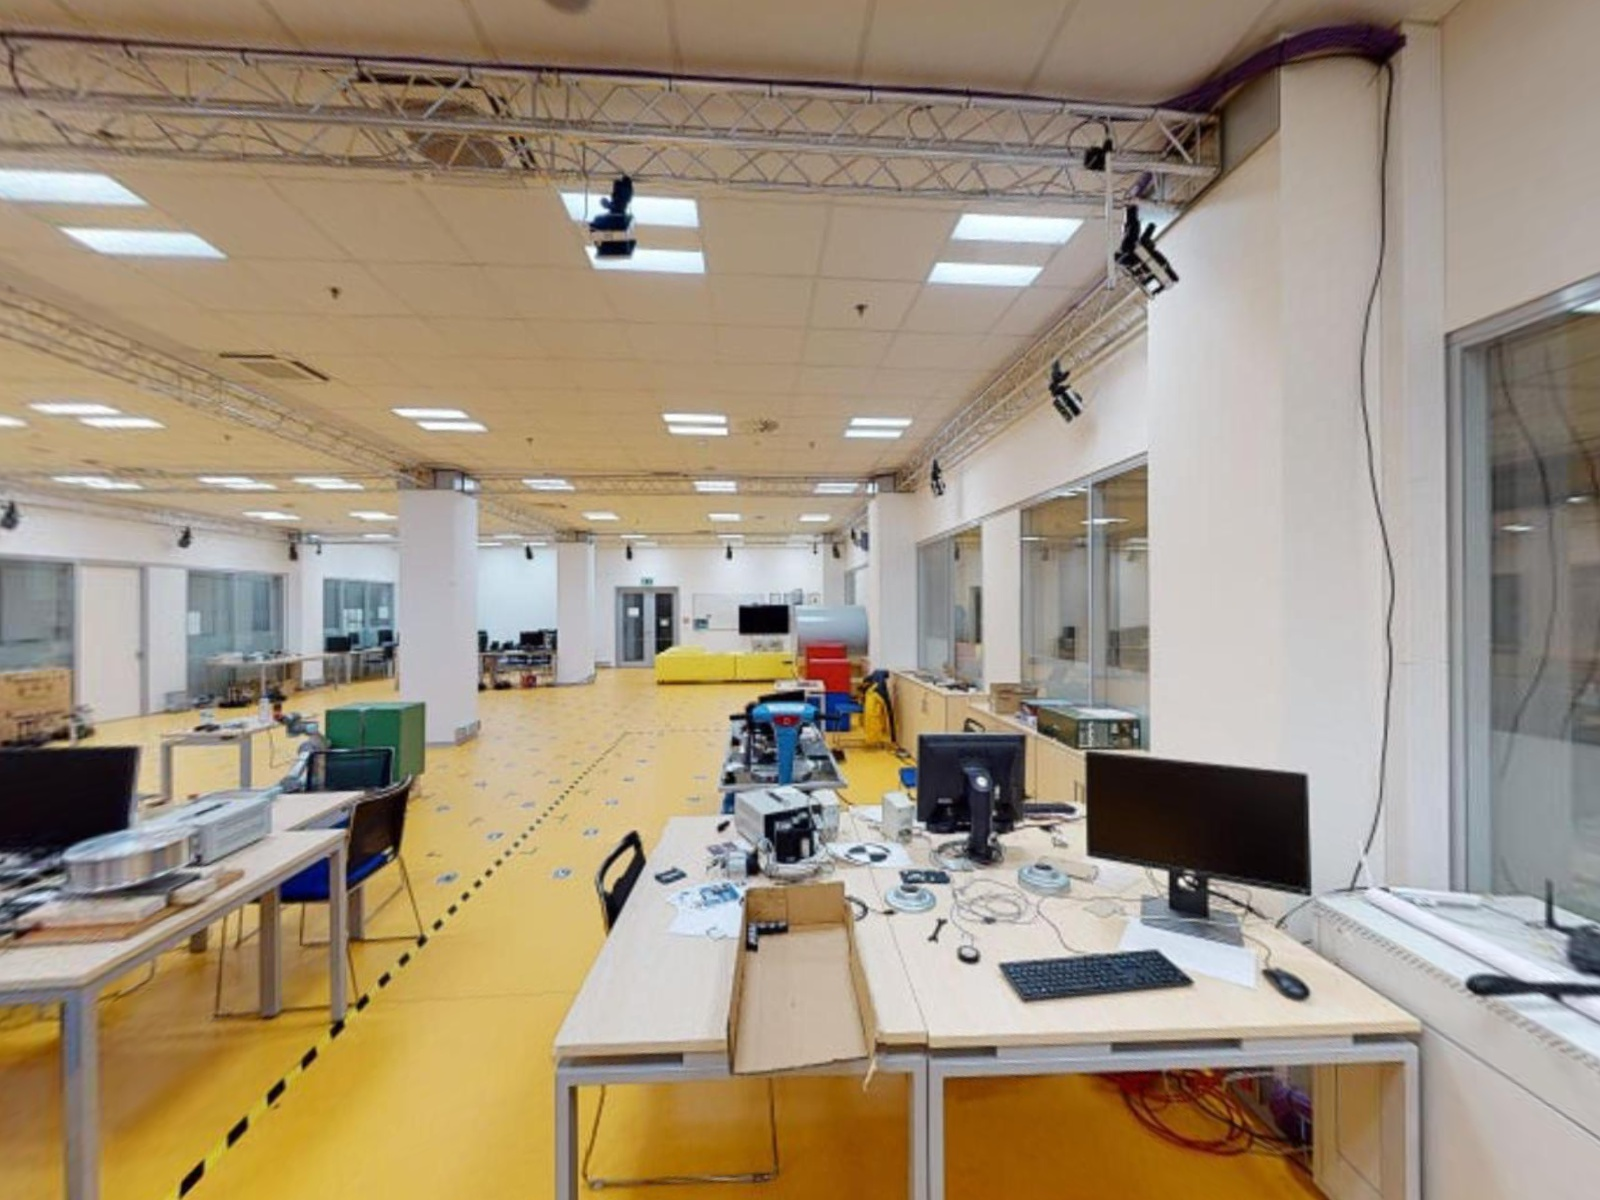
\includegraphics[width=0.8\textwidth]{cutout_19_-90_0_FoV106} \\
    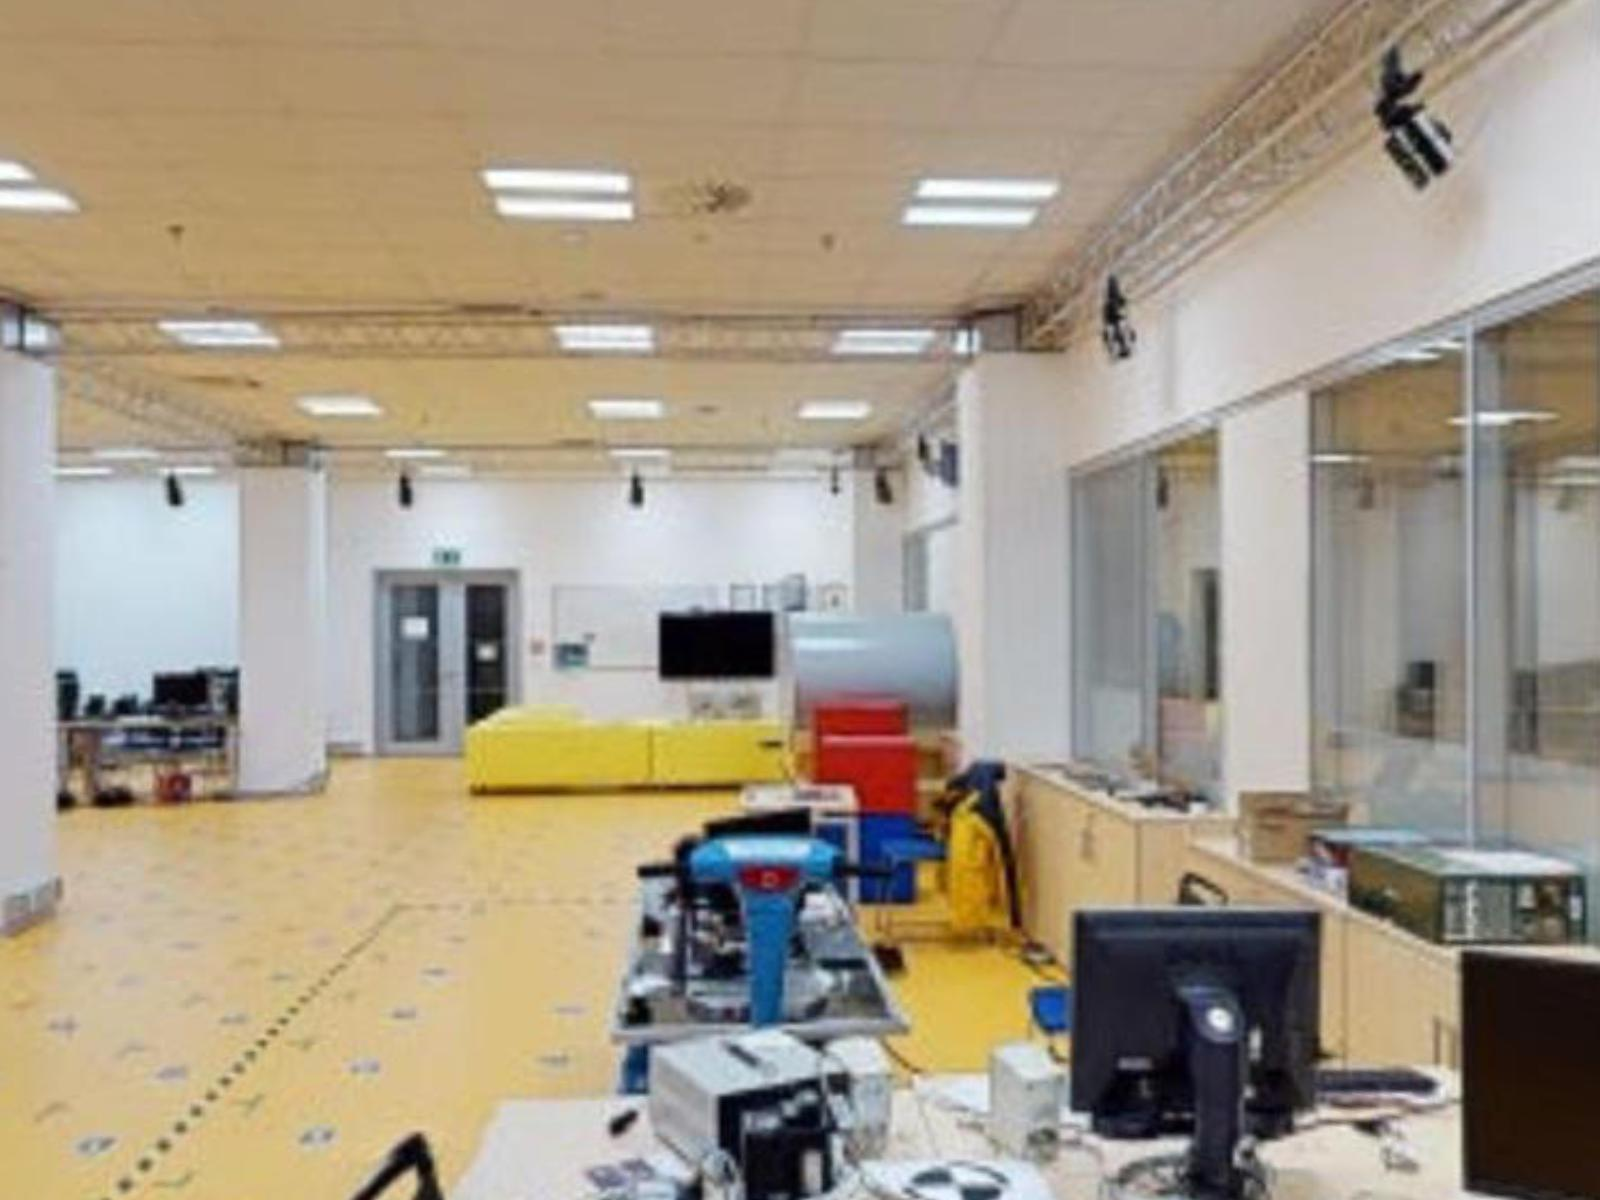
\includegraphics[width=0.8\textwidth]{cutout_19_-90_0_FoV60}
    \end{tabular}
	\caption{{\bf Visual quality comparision of the same cutout under different FoV.} Top: horizontal FoV: $106.26\degree$. Bottom: horizontal FoV: $60.00\degree$. The image with a lower FoV contains a lot of artifacts and is of lower visual quality.}
	\label{fig:fov-quality}
    }
\end{figure*}

TODO: how are reflective surfaces handled?

\chapter{Demo}

InLoc \cite{taira2018inloc} authors provide a demonstration in MATLAB that operates on the InLoc dataset. I have taken this demonstration and adjusted it, so that it works on the InLocCIIRC dataset instead. I have added an evaluation script, that was missing from the original code. Although the evaluation of InLoc is handled by \url{visuallocalization.net}, this tool of course doesn't handle the newly created InLocCIIRC dataset yet.

The entire InLocCIIRC demo has to run on a machine with a GPU. This is because we are using inference of NetVLAD neural network, which would take much longer on a CPU. This restriction is present in InLoc demo as well.

One difference from the original InLoc is that I am using a mesh model projection instead of a point cloud projection in the point verification step. This is because the code for point cloud projection did not support variable point size. Because the model is dense (compared to Faro 3D scanner), the projection can sometimes see through pillars or objects that are close to the camera. This is not desirable, as seeing what is behind the object can result in a different NetVLAD descriptor that is not similar to the query image.

\chapter{Evaluation}

In order to measure how the InLocCIIRC algorithm is performing, I have measured the percentage of correctly localized poses within a threshold from a reference pose. Position difference threshold is one of the following values, with decreasing difficulty: 0.25m, 0.50m, 1.00m. Angular threshold is set to 10\degree. Table \ref{tab:estimation-errors} shows the errors in pose estimation for individual queries. Rows with a NaN entry mean that densePE returned a NaN P matrix. Translation error $666.00$ signals that the estimated pose was in a different space than the reference query pose. Table \ref{tab:estimation-performance} shows the performance under the various thresholds. The InMap/OffMap performance is also shown. Figure \ref{fig:dist-thresh-vs-accuracy} shows how the localization accuracy changes given increasing translation error threshold.

\begin{table}
	\centering
	\begin{tabular}{|c|c|c|c|}
		\hline
		\bfseries Query ID & \bfseries InMap & \bfseries Translation [m] & \bfseries Orientation [\degree]
		\csvreader[head to column names]{evaluation/errors.csv}{}
		{\\ \hline \id & \inMap & \translation & \orientation}
		\\\hline
	\end{tabular}
	\caption{Pose estimation errors on query images.}
	\label{tab:estimation-errors}
\end{table}

Figure \ref{fig:queryPipeline} shows example queries, how they are being processed and what is the localization result.

\newcommand{\thiswidth}{0.19\linewidth} 
{
\setlength{\tabcolsep}{1pt}
\cellspacetoplimit 2pt
\cellspacebottomlimit 2pt
\begin{figure*}
    \centering
    {\footnotesize
	\begin{tabular}{Sc|Sc|Sc|Sc|Sc|}
	& Query image & Closest cutout & Synthesized view & Error map \\
	\hline
	\makecell{Query 3 \\ 1.36 m, 7.83$\degree$} &
    \adjincludegraphics[valign=M,width=\thiswidth]{evaluation/queryPipeline/3.jpg/query_3} &
	\adjincludegraphics[valign=M,width=\thiswidth]{evaluation/queryPipeline/3.jpg/chosen_cutout_B-315_19_90_0} &
    \adjincludegraphics[valign=M,width=\thiswidth]{evaluation/queryPipeline/3.jpg/synthesized} &
	\adjincludegraphics[valign=M,width=\thiswidth]{evaluation/queryPipeline/3.jpg/errmap} \\
	\hline
	\makecell{Query 6 \\ 0.34 m, 3.82$\degree$} &
    \adjincludegraphics[valign=M,width=\thiswidth]{evaluation/queryPipeline/6.jpg/query_6} &
    \adjincludegraphics[valign=M,width=\thiswidth]{evaluation/queryPipeline/6.jpg/chosen_cutout_B-315_2_90_0} &
    \adjincludegraphics[valign=M,width=\thiswidth]{evaluation/queryPipeline/6.jpg/synthesized} &
	\adjincludegraphics[valign=M,width=\thiswidth]{evaluation/queryPipeline/6.jpg/errmap} \\
	\hline
	\makecell{Query 31 \\ 0.65 m, 2.50$\degree$} &
    \adjincludegraphics[valign=M,width=\thiswidth]{evaluation/queryPipeline/31.jpg/query_31} &
    \adjincludegraphics[valign=M,width=\thiswidth]{evaluation/queryPipeline/31.jpg/chosen_cutout_B-315_4_30_0} &
    \adjincludegraphics[valign=M,width=\thiswidth]{evaluation/queryPipeline/31.jpg/synthesized} &
	\adjincludegraphics[valign=M,width=\thiswidth]{evaluation/queryPipeline/31.jpg/errmap} \\
	\hline
	\makecell{Query 38 \\ 0.13 m, 1.27$\degree$} &
    \adjincludegraphics[valign=M,width=\thiswidth]{evaluation/queryPipeline/38.jpg/query_38} &
    \adjincludegraphics[valign=M,width=\thiswidth]{evaluation/queryPipeline/38.jpg/chosen_cutout_B-315_2_-120_-30} &
    \adjincludegraphics[valign=M,width=\thiswidth]{evaluation/queryPipeline/38.jpg/synthesized} &
	\adjincludegraphics[valign=M,width=\thiswidth]{evaluation/queryPipeline/38.jpg/errmap} \\
	\hline
	\makecell{Query 16 \\ 19.74 m, 177.21$\degree$} &
    \adjincludegraphics[valign=M,width=\thiswidth]{evaluation/queryPipeline/16.jpg/query_16} &
    \adjincludegraphics[valign=M,width=\thiswidth]{evaluation/queryPipeline/16.jpg/chosen_cutout_B-315_16_-180_-30} &
    \adjincludegraphics[valign=M,width=\thiswidth]{evaluation/queryPipeline/16.jpg/synthesized} &
	\adjincludegraphics[valign=M,width=\thiswidth]{evaluation/queryPipeline/16.jpg/errmap} \\
	\hline
	\makecell{Query 26 \\ 6.09 m, 179.05$\degree$} &
    \adjincludegraphics[valign=M,width=\thiswidth]{evaluation/queryPipeline/26.jpg/query_26} &
    \adjincludegraphics[valign=M,width=\thiswidth]{evaluation/queryPipeline/26.jpg/chosen_cutout_B-315_10_-90_-30} &
    \adjincludegraphics[valign=M,width=\thiswidth]{evaluation/queryPipeline/26.jpg/synthesized} &
	\adjincludegraphics[valign=M,width=\thiswidth]{evaluation/queryPipeline/26.jpg/errmap} \\
	\hline
    \end{tabular}
    \caption{{\bf Qualitative comparison of query localization.} From left to right: Query name and localization error (meters, degrees), query image, the best matching database image, synthesized view at the estimated pose, error map between the query image and the synthesized view. Green dots are the inlier matches obtained by P3P-LO-RANSAC. The query images in the 1st, 2nd, 3th and 4th row are well localized within 1.5 meters and 10.0 degrees whereas localization results in the last two rows are incorrect. All of the shown queries are OffMap, to test challenging estimation scenarios.
    \label{fig:queryPipeline}}
    }
\end{figure*}
}

\begin{table}
	\centering
	\begin{tabular}{|c|c||c|c|c|}
		\hline
		Threshold & InLoc & \bfseries InLocCIIRC & InMap & OffMap \\
		\hline
		0.25m & 38.9\% & \bfseries 47.5\% & 80.00\% & 42.86\% \\
		0.50m & 56.5\% & \bfseries 57.5\% & 100.00\% & 51.43\% \\
		1.00m & \bfseries 69.9\% & 62.5\% & 100.00\% & 57.14\% \\
		\hline
	\end{tabular}
	\caption{Evaluation of performance of localization methods. The method in the first column was run on InLoc dataset. The second column method was run on InLocCIIRC dataset. Percentage rate of correctly localized queries within given threshold is shown. Angular threshold is equal to $10\degree$ in every row. The last two columns belong to InLocCIIRC method. InMap queries are queries for which we have a similar cutout in the dataset.}
	\label{tab:estimation-performance}
\end{table}

\begin{figure}
	\centering
	% GNUPLOT: LaTeX picture with Postscript
\begingroup
  \makeatletter
  \providecommand\color[2][]{%
    \GenericError{(gnuplot) \space\space\space\@spaces}{%
      Package color not loaded in conjunction with
      terminal option `colourtext'%
    }{See the gnuplot documentation for explanation.%
    }{Either use 'blacktext' in gnuplot or load the package
      color.sty in LaTeX.}%
    \renewcommand\color[2][]{}%
  }%
  \providecommand\includegraphics[2][]{%
    \GenericError{(gnuplot) \space\space\space\@spaces}{%
      Package graphicx or graphics not loaded%
    }{See the gnuplot documentation for explanation.%
    }{The gnuplot epslatex terminal needs graphicx.sty or graphics.sty.}%
    \renewcommand\includegraphics[2][]{}%
  }%
  \providecommand\rotatebox[2]{#2}%
  \@ifundefined{ifGPcolor}{%
    \newif\ifGPcolor
    \GPcolorfalse
  }{}%
  \@ifundefined{ifGPblacktext}{%
    \newif\ifGPblacktext
    \GPblacktexttrue
  }{}%
  % define a \g@addto@macro without @ in the name:
  \let\gplgaddtomacro\g@addto@macro
  % define empty templates for all commands taking text:
  \gdef\gplbacktext{}%
  \gdef\gplfronttext{}%
  \makeatother
  \ifGPblacktext
    % no textcolor at all
    \def\colorrgb#1{}%
    \def\colorgray#1{}%
  \else
    % gray or color?
    \ifGPcolor
      \def\colorrgb#1{\color[rgb]{#1}}%
      \def\colorgray#1{\color[gray]{#1}}%
      \expandafter\def\csname LTw\endcsname{\color{white}}%
      \expandafter\def\csname LTb\endcsname{\color{black}}%
      \expandafter\def\csname LTa\endcsname{\color{black}}%
      \expandafter\def\csname LT0\endcsname{\color[rgb]{1,0,0}}%
      \expandafter\def\csname LT1\endcsname{\color[rgb]{0,1,0}}%
      \expandafter\def\csname LT2\endcsname{\color[rgb]{0,0,1}}%
      \expandafter\def\csname LT3\endcsname{\color[rgb]{1,0,1}}%
      \expandafter\def\csname LT4\endcsname{\color[rgb]{0,1,1}}%
      \expandafter\def\csname LT5\endcsname{\color[rgb]{1,1,0}}%
      \expandafter\def\csname LT6\endcsname{\color[rgb]{0,0,0}}%
      \expandafter\def\csname LT7\endcsname{\color[rgb]{1,0.3,0}}%
      \expandafter\def\csname LT8\endcsname{\color[rgb]{0.5,0.5,0.5}}%
    \else
      % gray
      \def\colorrgb#1{\color{black}}%
      \def\colorgray#1{\color[gray]{#1}}%
      \expandafter\def\csname LTw\endcsname{\color{white}}%
      \expandafter\def\csname LTb\endcsname{\color{black}}%
      \expandafter\def\csname LTa\endcsname{\color{black}}%
      \expandafter\def\csname LT0\endcsname{\color{black}}%
      \expandafter\def\csname LT1\endcsname{\color{black}}%
      \expandafter\def\csname LT2\endcsname{\color{black}}%
      \expandafter\def\csname LT3\endcsname{\color{black}}%
      \expandafter\def\csname LT4\endcsname{\color{black}}%
      \expandafter\def\csname LT5\endcsname{\color{black}}%
      \expandafter\def\csname LT6\endcsname{\color{black}}%
      \expandafter\def\csname LT7\endcsname{\color{black}}%
      \expandafter\def\csname LT8\endcsname{\color{black}}%
    \fi
  \fi
    \setlength{\unitlength}{0.0500bp}%
    \ifx\gptboxheight\undefined%
      \newlength{\gptboxheight}%
      \newlength{\gptboxwidth}%
      \newsavebox{\gptboxtext}%
    \fi%
    \setlength{\fboxrule}{0.5pt}%
    \setlength{\fboxsep}{1pt}%
\begin{picture}(7200.00,5040.00)%
    \gplgaddtomacro\gplbacktext{%
      \csname LTb\endcsname%%
      \put(1619,704){\makebox(0,0)[r]{\strut{}$0$}}%
      \csname LTb\endcsname%%
      \put(1619,1733){\makebox(0,0)[r]{\strut{}$20$}}%
      \csname LTb\endcsname%%
      \put(1619,2762){\makebox(0,0)[r]{\strut{}$40$}}%
      \csname LTb\endcsname%%
      \put(1619,3790){\makebox(0,0)[r]{\strut{}$60$}}%
      \csname LTb\endcsname%%
      \put(1619,4819){\makebox(0,0)[r]{\strut{}$80$}}%
      \csname LTb\endcsname%%
      \put(1751,484){\makebox(0,0){\strut{}$0$}}%
      \csname LTb\endcsname%%
      \put(2265,484){\makebox(0,0){\strut{}$0.25$}}%
      \csname LTb\endcsname%%
      \put(2780,484){\makebox(0,0){\strut{}$0.5$}}%
      \csname LTb\endcsname%%
      \put(3294,484){\makebox(0,0){\strut{}$0.75$}}%
      \csname LTb\endcsname%%
      \put(3809,484){\makebox(0,0){\strut{}$1$}}%
      \csname LTb\endcsname%%
      \put(4323,484){\makebox(0,0){\strut{}$1.25$}}%
      \csname LTb\endcsname%%
      \put(4837,484){\makebox(0,0){\strut{}$1.5$}}%
      \csname LTb\endcsname%%
      \put(5352,484){\makebox(0,0){\strut{}$1.75$}}%
      \csname LTb\endcsname%%
      \put(5866,484){\makebox(0,0){\strut{}$2$}}%
    }%
    \gplgaddtomacro\gplfronttext{%
      \csname LTb\endcsname%%
      \put(1146,2761){\rotatebox{-270}{\makebox(0,0){\strut{}Correctly localized queries [\%]}}}%
      \put(3808,154){\makebox(0,0){\strut{}Distance threshold [meters]}}%
      \csname LTb\endcsname%%
      \put(5011,1623){\makebox(0,0)[r]{\strut{}InLoc}}%
      \csname LTb\endcsname%%
      \put(5011,1403){\makebox(0,0)[r]{\strut{}InLocCIIRC}}%
    }%
    \gplbacktext
    \put(0,0){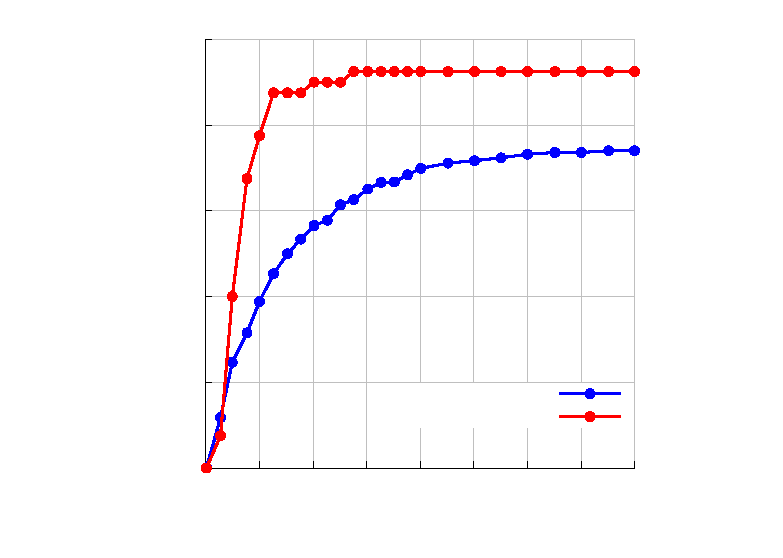
\includegraphics{distThreshVsAccuracy}}%
    \gplfronttext
  \end{picture}%
\endgroup

	\caption{Comparison between InLoc and InLocCIIRC on their respective datasets. The x-axis describes the maximum allowed translation error. The angular threshold is set to $10\degree$.}
	\label{fig:dist-thresh-vs-accuracy}
\end{figure}

Figures \ref{fig:topView-B-315} and \ref{fig:topView-B-670} depict the dataset including the localization results.

\begin{figure}
	\centering
 	\includegraphics[width=0.65\textwidth]{evaluation/topView-B-315}
 	\caption{View on the floor plan of room B-315. Red dots: sweeps. Blue dots: queries. Yellow dots: estimated query poses.}
 	\label{fig:topView-B-315}
\end{figure} 

\begin{figure}
	\centering
 	\includegraphics[width=0.65\textwidth]{evaluation/topView-B-670}
 	\caption{View on the floor plan of room B-670. Red dots: sweeps. Blue dots: queries. Yellow dots: estimated query poses. Queries 23 and 40 from room B-315 were incorrectly localized. They are positioned to the left side of this floor plan, but they are not drawn, in order to simplify this figure.}
 	\label{fig:topView-B-670}
\end{figure} 

\appendix

\printindex

\appendix

%\bibliographystyle{amsalpha}
\bibliographystyle{iso690}
\bibliography{bibliography}

\ctutemplate{specification.as.chapter}

\end{document}